\documentclass[10pt]{article}
\usepackage[portuguese]{babel}
\usepackage[utf8]{inputenc}
\usepackage[pdftex]{graphicx}
\usepackage{venndiagram}
\usepackage{subcaption}
\usepackage{caption}
\usepackage[backend=biber,style=authoryear-ibid]{biblatex}
\usepackage[normalem]{ulem}
\usepackage[margin=0.8in]{geometry}
%\addbibresource{}
\graphicspath{{Pictures/}}
\usepackage{tikz}
\usepackage{setspace}
\usepackage{enumitem}
\usepackage{textcomp}
\usepackage{listings}
\usepackage{float}


\author{}
\title{}
\date{}

\newcommand{\quotebox}[3]{
  \begin{center}
\noindent\fbox{ 
  \parbox{#3\textwidth}{%
  {\itshape#1\itshape}

  \raggedleft {\textbf{#2}} 
    }%  
}
\end{center}
}

\newcommand{\spawnfig}[3]
{
  \begin{figure}[h]
  \centering
  \includegraphics[scale={#3}]{#1}
  \caption{#2}
  \end{figure}
}

\definecolor{dkgreen}{rgb}{0,0.6,0}
\definecolor{gray}{rgb}{0.5,0.5,0.5}
\definecolor{mauve}{rgb}{0.58,0,0.82}

\lstset{frame=tb,
  language=C,
  aboveskip=2mm,
  belowskip=2mm,
  showstringspaces=false,
  columns=flexible,
  basicstyle={\small\ttfamily},
  numbers=none,
  numberstyle=\tiny\color{gray},
  keywordstyle=\color{blue},
  commentstyle=\color{dkgreen},
  stringstyle=\color{mauve},
  breaklines=true,
  breakatwhitespace=true,
  tabsize=3
}

\begin{document}
\maketitle

\section{Program Scope}

The program should be able to receive as input a chess move in UCI(Universal
Chess Interface) format i.e
e2e4, and if the movement is valid, output the board state to the user or inform
the user the input isn't valid. For this matter, the standard python libraries is
enough address the problem. For debugging purposes, a graphical interface was
also required and implemented in pygame, a graphical framework for games. Also
for preparing the tests, it was used the program
\textit{pgn-extract} to convert PGN game notation to UCI notation, although, not
necessary for running nor testing. For running the tests, pytest was used.


\section{Program project}

The project is constituted by four modules that contains in itself their
respective major class: The Piece, Board, Chess and GUI classes, which can be
described as:
\begin{enumerate}
    \item The \textbf{Pieces} module contains the Piece class, that is inherited by all
        the chess pieces, and specify how to get from each piece their own set
        of possible moves, where they are on the board, and what to do with
        the board when what to do when the piece moves.
        \item The \textbf{Board} module contains the Board class that is used to save and
            process all
            information relative to board state, such as pieces positions,
            castling rights, number of turns, \textit{En Passeant} possibility, etc.
            And with that it information it can save and load the board state
            in the form of a FEN(Forsyth–Edwards
            Notation)\footnote{\url{https://en.wikipedia.org/wiki/Forsyth\%E2\%80\%93Edwards_Notation}}
        \item The \textbf{Chess} module contains the Chess class that is used to process
            the Board information and create legal moves from which the player
            can chose to play.
        \item The \textbf{GUI} module contains the GUI class which uses the Board and Chess classes to play the game in a graphical interface mode.
\end{enumerate}


\begin{figure}[H]
    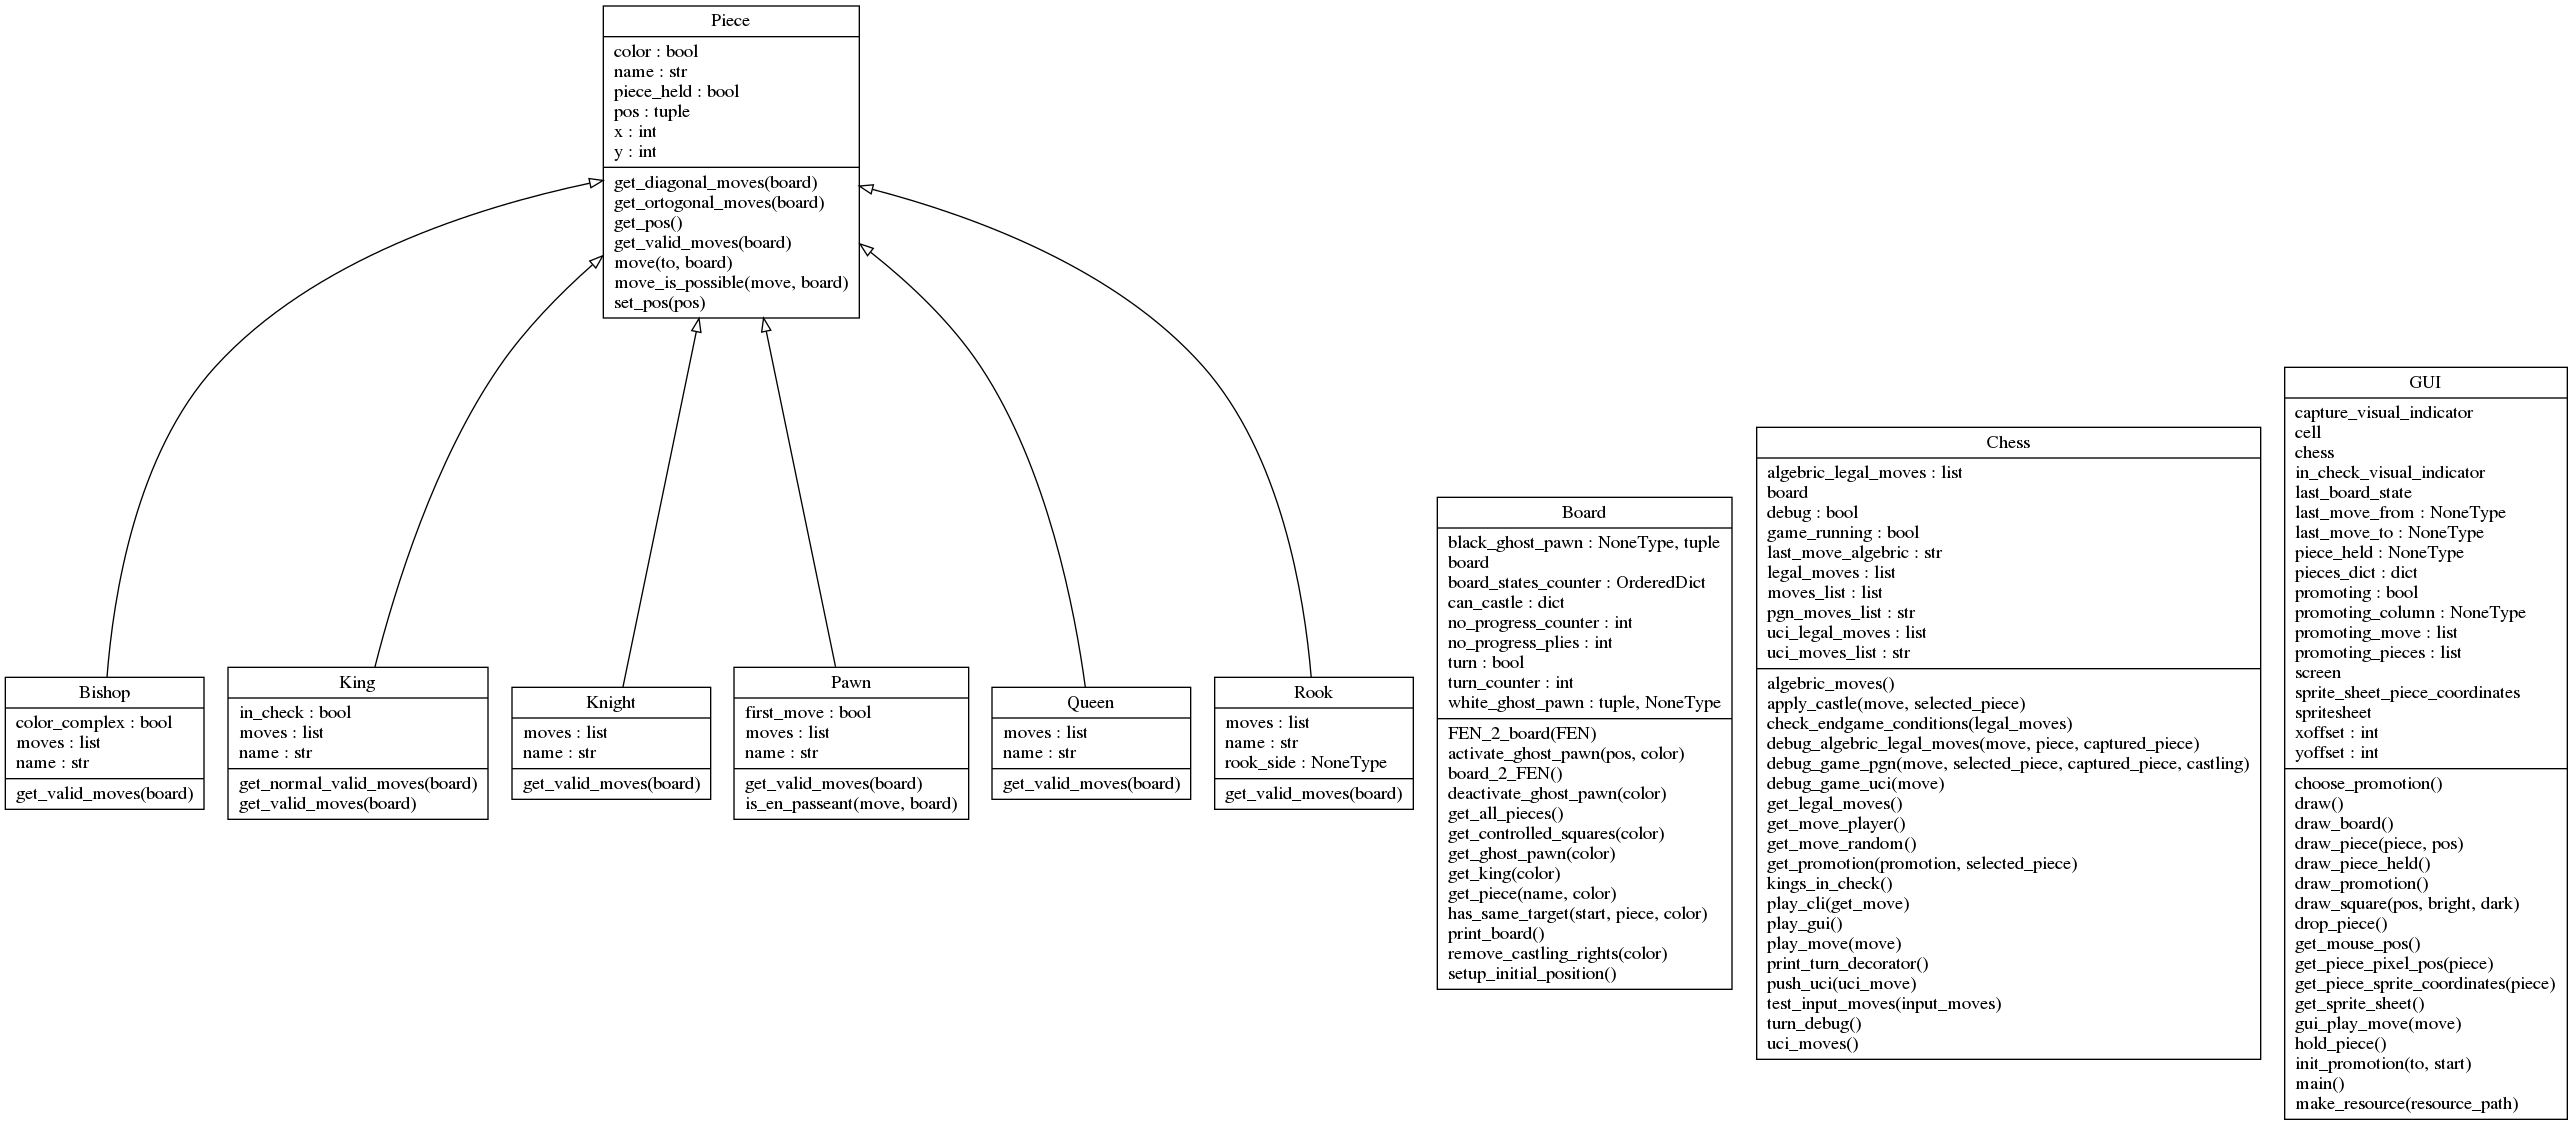
\includegraphics[scale=0.2]{fig/classes_Chess.png}
\end{figure}


\section{Testing}

Three approaches were made to certify the accuracy of the game:

\begin{enumerate}[label=\arabic*)]
\item Brute force the initial position and compare with the Shannon's
    Calculations, which stands for a proof table of the total possible moves
    that can arise within a certain ply(half-move)
\item Brute force ``complex positions'' and comparing with a proof table of possible
    moves(Same approach as above, but not from the initial position).
\item Specific tests to test draw conditions
\end{enumerate}

To execute all the tests we run the following command at the top level directory
of the project, i.e ``/mychess''
\begin{lstlisting}
pytests tests
\end{lstlisting}

or for specific tests, we can also run for example:

\begin{lstlisting}
pytests tests/testdraw.py
\end{lstlisting}

The result of both tests will be located at ``mychess/logs''


\subsection{Shannon's Calculation}


\begin{table}[H]
\center
\begin{tabular}{|c|c|}
\hline
\textbf{Number of plies (half-moves)}  & \textbf{Number of possible games}  \\
\hline
  1   & 20 \\
\hline
   2  &  400 \\
\hline
  3   & 8092 \\
\hline
4  & 197,281 \\
\hline
5   & 4,865,609 \\
\hline
6   & 119,060,324 \\
\hline
\ldots & \ldots \\
\hline
10 & 69,352,859,712,417 \\
\hline
\end{tabular}
\caption{Shannon's Calculation. Obs: A turn is composed by a white move and a
    black move. A ply is half-move, therefore five plies
stands for white playing three times and black two.}
\end{table}

For testing basic moves correctness, it was used the Shannon's Calculation,
which stands for all the possible moves that can be played until a certain
ply(half-move). By the limitations of the computer power available at our
disposal, and considering that the game was not written in a language nor
written in a way for fast computation, we could only check the precision of the
game until 5 ply, as we can see by the test log:
\begin{lstlisting}
2022-01-22 00:00:36,742 Result of possible games with 1 ply: 20/20 - OK
2022-01-22 00:00:36,742 Elapsed time in 1 ply: 00h00m00s seconds
2022-01-22 00:00:37,312 Result of possible games with 2 ply: 400/400 - OK
2022-01-22 00:00:37,312 Elapsed time in 2 ply: 00h00m00s seconds
2022-01-22 00:00:52,137 Result of possible games with 3 ply: 8902/8902 - OK
2022-01-22 00:00:52,137 Elapsed time in 3 ply: 00h00m14s seconds
2022-01-22 00:07:11,715 Result of possible games with 4 ply: 197281/197281 - OK
2022-01-22 00:07:11,715 Elapsed time in 4 ply: 00h06m19s seconds
2022-01-22 08:45:00,073 Result of possible games with 5 ply: 4865609/4865609 - OK
2022-01-22 08:45:00,073 Elapsed time in 5 ply: 08h37m48s seconds
    
\end{lstlisting}

Although this is a good signal that basic operations are working, in 5 plies we
cannot test all the complications that might arise during a chess game.

\begin{table}[H]
\center
\begin{tabular}{|c|c|c|c|c|c|c|c|c|}
\hline
\textbf{Depth}   & \textbf{Captures} & \textbf{E.P} &
\textbf{Castles} & \textbf{Promotions} & \textbf{Checks} & \textbf{Dscry
Checks} & \textbf{Dbl Checks} & \textbf{Checkmates} \\
\hline
   1  & 0 & 0 & 0 & 0 & 0 & 0 & 0 & 0 \\
\hline
   2  & 0 & 0 & 0 & 0 & 0 & 0 & 0 & 0 \\
\hline
   3  & 34 & 0 & 0 & 0 & 12 & 0 & 0 & 0 \\
\hline
   4  & 1576 & 0 & 0 & 0 & 469 & 0 & 0 & 8 \\
\hline
5  & 82,719 & 258 & 0 & 0 & 27,251 & 6 & 0 & 347 \\
\hline
\end{tabular}
\caption{Number of ``special'' moves by depth accordingly to
\url{https://www.chessprogramming.org/Perft_Results} }
\end{table}

By this table we can see that we need to concentrate our efforts in testing
Castle, Promotions, Discovery Checks and Double Checks. Because they don't arise
until moves later than 5.

\subsection{Brute forcing complex positions}


One way to test them, is loading ``complex positions'', which contain in its
possibilities: Castling, promotion, discovery checks and double checks, brute
force their
possible moves, and compare the results with a proof table. Using the
positions recommended in \url{https://www.chessprogramming.org/Perft_Results},
with their respective proof table,
we get the following result from 5 ``complex positions'':

\begin{lstlisting}
>>> $ pytest -k ''test_position''
12:12:49 ----------------------------------------
12:12:49 Initiating move generation test on depth: 3
12:12:49 FEN of position to be brute forced:r3k2r/p1ppqpb1/bn2pnp1/3PN3/1p2P3/2N2Q1p/PPPBBPPP/R3K2R w KQkq - 0 0
12:12:50 Result of possible games with 1 ply: 48/48 - OK
12:12:50 Elapsed time in 1 ply: 00h00m00s seconds
12:12:54 Result of possible games with 2 ply: 2039/2039 - OK
12:12:54 Elapsed time in 2 ply: 00h00m04s seconds
12:16:26 Result of possible games with 3 ply: 97862/97862 - OK
12:16:26 Elapsed time in 3 ply: 00h03m32s seconds
12:16:26 TEST SUCCESSFUL
12:16:26 Total Elapsed time: (00h03m36s)
12:16:26 ----------------------------------------
12:16:26 Initiating move generation test on depth: 4
12:16:26 FEN of position to be brute forced:8/2p5/3p4/KP5r/1R3p1k/8/4P1P1/8 w - - 0 0
12:16:26 Result of possible games with 1 ply: 14/14 - OK
12:16:26 Elapsed time in 1 ply: 00h00m00s seconds
12:16:26 Result of possible games with 2 ply: 191/191 - OK
12:16:26 Elapsed time in 2 ply: 00h00m00s seconds
12:16:29 Result of possible games with 3 ply: 2812/2812 - OK
12:16:29 Elapsed time in 3 ply: 00h00m03s seconds
12:17:19 Result of possible games with 4 ply: 43238/43238 - OK
12:17:19 Elapsed time in 4 ply: 00h00m49s seconds
12:17:19 TEST SUCCESSFUL
12:17:19 Total Elapsed time: (00h00m53s)
12:17:19 ----------------------------------------
12:17:19 Initiating move generation test on depth: 4
12:17:19 FEN of position to be brute forced:r3k2r/Pppp1ppp/1b3nbN/nP6/BBP1P3/q4N2/Pp1P2PP/R2Q1RK1 w kq - 0 1
12:17:19 Result of possible games with 1 ply: 6/6 - OK
12:17:19 Elapsed time in 1 ply: 00h00m00s seconds
12:17:20 Result of possible games with 2 ply: 264/264 - OK
12:17:20 Elapsed time in 2 ply: 00h00m00s seconds
12:17:39 Result of possible games with 3 ply: 9467/9467 - OK
12:17:39 Elapsed time in 3 ply: 00h00m19s seconds
12:34:01 Result of possible games with 4 ply: 422333/422333 - OK
12:34:01 Elapsed time in 4 ply: 00h16m21s seconds
12:34:01 TEST SUCCESSFUL
12:34:01 Total Elapsed time: (00h16m41s)
12:34:01 ----------------------------------------
12:34:01 Initiating move generation test on depth: 4
12:34:01 FEN of position to be brute forced:rnbq1k1r/pp1Pbppp/2p5/8/2B5/8/PPP1NnPP/RNBQK2R w KQ - 1 8
12:34:01 Result of possible games with 1 ply: 44/44 - OK
12:34:01 Elapsed time in 1 ply: 00h00m00s seconds
12:34:04 Result of possible games with 2 ply: 1486/1486 - OK
12:34:04 Elapsed time in 2 ply: 00h00m02s seconds
12:36:04 Result of possible games with 3 ply: 62379/62379 - OK
12:36:04 Elapsed time in 3 ply: 00h02m00s seconds
14:39:42 Result of possible games with 4 ply: 2103487/2103487 - OK
14:39:42 Elapsed time in 4 ply: 02h03m37s seconds
14:39:42 TEST SUCCESSFUL
14:39:42 Total Elapsed time: (02h05m41s)
14:39:42 ----------------------------------------
14:39:42 Initiating move generation test on depth: 3
14:39:42 FEN of position to be brute forced:r4rk1/1pp1qppp/p1np1n2/2b1p1B1/2B1P1b1/P1NP1N2/1PP1QPPP/R4RK1 w - - 0 10
14:39:43 Result of possible games with 1 ply: 46/46 - OK
14:39:43 Elapsed time in 1 ply: 00h00m00s seconds
14:39:47 Result of possible games with 2 ply: 2079/2079 - OK
14:39:47 Elapsed time in 2 ply: 00h00m04s seconds
14:43:04 Result of possible games with 3 ply: 89890/89890 - OK
14:43:04 Elapsed time in 3 ply: 00h03m17s seconds
14:43:04 TEST SUCCESSFUL
14:43:04 Total Elapsed time: (00h03m21s)
    
\end{lstlisting}

By doing these tests, we can be relatively certain that the ``special moves'' are working
as desired.

\subsection{Specific tests for Draws}

Given that draws take so long to happen, they very rarely appear in brute forcing
tests. Having that in mind, we made specific tests that checks all the draw
conditions.  For example, we feed this list of moves: 

\begin{lstlisting}

movedraw50 = ["d2d4 g8f6 c2c4 g7g6 b1c3 f8g7 e2e4 d7d6 g1f3 e8g8 f1e2 e7e5 e1g1
b8c6 d4d5 c6e7 f3d2 a7a5 a1b1 f6d7 a2a3 f7f5 b2b4 g8h8 f2f3 e7g8 d1c2 g8f6 c3b5
a5b4 a3b4 f6h5 g2g3 d7f6 c4c5 c8d7 b1b3 h5g3 h2g3 f6h5 f3f4 e5f4 c5c6 b7c6 d5c6
h5g3 b3g3 f4g3 c6d7 g3g2 f1f3 d8d7 c1b2 f5e4 f3f8 a8f8 b2g7 d7g7 c2e4 g7f6 d2f3
f6f4 e4e7 f8f7 e7e6 f7f6 e6e8 f6f8 e8e7 f8f7 e7e6 f7f6 e6b3 g6g5 b5c7 g5g4 c7d5
f4c1 b3d1 c1d1 e2d1 f6f5 d5e3 f5f4 f3e1 f4b4 d1g4 h7h5 g4f3 d6d5 e3g2 h5h4 e1d3
b4a4 g2f4 h8g7 g1g2 g7f6 f3d5 a4a5 d5c6 a5a6 c6b7 a6a3 b7e4 a3a4 e4d5 a4a5 d5c6
a5a6 c6f3 f6g5 f3b7 a6a1 b7c8 a1a4 g2f3 a4c4 c8d7 g5f6 f3g4 c4d4 d7c6 d4d8 g4h4
d8g8 c6e4 g8g1 f4h5 f6e6 h5g3 e6f6 h4g4 g1a1 e4d5 a1a5 d5f3 a5a1 g4f4 f6e6 d3c5
e6d6 g3e4 d6e7 f4e5 a1f1 f3g4 f1g1 g4e6 g1e1 e6c8 e1c1 e5d4 c1d1 c5d3 e7f7 d4e3
d1a1 e3f4 f7e7 d3b4 a1c1 b4d5 e7f7 c8d7 c1f1 f4e5 f1a1 e4g5 f7g6 g5f3 g6g7 d7g4
g7g6 d5f4 g6g7 f3d4 a1e1 e5f5 e1c1 g4e2 c1e1 e2h5 e1a1 f4e6 g7h6 h5e8 a1a8 e8c6
a8a1 f5f6 h6h7 e6g5 h7h8 d4e6 a1a6 c6e8 a6a8 e8h5 a8a1 h5g6 a1f1 f6e7 f1a1 g5f7
h8g8 f7h6 g8h8 h6f5 a1a7 e7f6 a7a1 f5e3 a1e1 e3d5 e1g1 g6f5 g1f1 d5f4 f1a1 f4g6
h8g8 g6e7 g8h8 e6g5", "7k/4N3/5K2/5BN1/8/8/8/r7 b - - 100 113"]

\end{lstlisting}

Into our specific test function:

\begin{lstlisting}
    for test in tests:

        chess = Chess()
        fen = chess.test_input_moves(test[0].split(" "))
        r = fen == test[1]
        result = "OK" if r else "ERROR"
        logging.info(f"Test with fen {test[1]} resulted in: {result}")
        assert r

    logging.info(f"DRAW TEST SUCCESSFUL")

\end{lstlisting}

The test plays the game move by move, and prints the result of the comparison between the expected board state
result(FEN) with the FEN given by our function call. If our game returns the
exact expected FEN, the test was successful.

Similar tests were made with:
\begin{enumerate}[label=\arabic*)]
\item Insufficient material
    \begin{enumerate}[label=\arabic{enumii}.\arabic*)]
    \item Opposite colors bishops draw
    \item Knight and King vs King
    \item Bishop and King vs King
    \item King vs King
    \end{enumerate}
    
    \item Stalemate 
    \item Three Fold Repetition
    \item 50 move without pawn move or capture
\end{enumerate}

And their result can be found on the log:
\begin{lstlisting}

>>> $ pytest tests/test_draws.py
17:00:16 ----------------------------------------
17:00:17 Test with fen 7k/4N3/5K2/5BN1/8/8/8/r7 b - - 100 113 resulted in: OK
17:00:17 Test with fen rnbq1bnr/ppppkppp/8/4p3/4P3/8/PPPPKPPP/RNBQ1BNR w - - 10 7 resulted in: OK
17:00:17 Test with fen 6k1/6p1/7p/8/1p6/p1qp4/8/3K4 w - - 0 45 resulted in: OK
17:00:18 Test with fen 8/8/7k/8/8/8/8/n4K2 w - - 0 172 resulted in: OK
17:00:20 Test with fen 8/8/8/6k1/8/5K2/8/8 w - - 0 158 resulted in: OK
17:00:20 DRAW TEST SUCCESSFUL

\end{lstlisting}

With all these tests, we can be relatively sure that the game will be successfully
executed in the great majority of cases.



\section{User Docs}

\subsection{Installation}

Assuming you already have installed python and pip, the user only needs to run
the following command inside the top directory of the project:
\begin{lstlisting}
python3 -m pip install -e .
\end{lstlisting}

\textbf{If something in installation fails, the user might need to change directory to
        ``mychess/src'' and import the module and/or run the following execution options
        from there.}

\subsection{Usage}

There are three ways to interact with this program, by directly calling their
functions in the interpreter, or in a script, by calling the $play\_cli()$ or the
$play\_gui()$ functions. 

\subsubsection{Interpreter}

By running the program as a module, we can have a more flexible execution,
choosing what to be shown at which time. Below we have an example execution,
that uses all the necessary calls to obtain the same result as the other
execution options i.e CLI or GUI.

The calls are:

\begin{enumerate}[label=\arabic*)]
\item Chess() -- Creates game object
\item uci\_moves() -- Shows possible moves
\item push\_uci() -- Makes a move
\end{enumerate}



\begin{lstlisting}

>>> from mychess import *

>>> game = Chess()
Whites turn to move!
 *********************************
8| r | n | b | q | k | b | n | r |
7| p | p | p | p | p | p | p | p |
6|   |   |   |   |   |   |   |   |
5|   |   |   |   |   |   |   |   |
4|   |   |   |   |   |   |   |   |
3|   |   |   |   |   |   |   |   |
2| P | P | P | P | P | P | P | P |
1| R | N | B | Q | K | B | N | R |
   a   b   c   d   e   f   g   h
*********************************

# Make moves
>>> game.uci_moves()
a2a4 a2a3 b2b4 b2b3 b1c3 b1a3 c2c4 c2c3 d2d4 d2d3 e2e4 e2e3 f2f4 f2f3 g2g4 g2g3 g1h3 g1f3 h2h4 h2h3

>>> game.push_uci("e2e4")

Blacks turn to move!
*********************************
8| r | n | b | q | k | b | n | r |
7| p | p | p | p | p | p | p | p |
6|   |   |   |   |   |   |   |   |
5|   |   |   |   |   |   |   |   |
4|   |   |   |   | P |   |   |   |
3|   |   |   |   |   |   |   |   |
2| P | P | P | P |   | P | P | P |
1| R | N | B | Q | K | B | N | R |
   a   b   c   d   e   f   g   h
*********************************

>>> game = Chess("r3k2r/p1ppqpb1/bn2pnp1/3PN3/1p2P3/2N2Q1p/PPPBBPPP/R3K2R w KQkq - 0 0")
Whites turn to move!
*********************************
8| r |   |   |   | k |   |   | r |
7| p |   | p | p | q | p | b |   |
6| b | n |   |   | p | n | p |   |
5|   |   |   | P | N |   |   |   |
4|   | p |   |   | P |   |   |   |
3|   |   | N |   |   | Q |   | p |
2| P | P | P | B | B | P | P | P |
1| R |   |   |   | K |   |   | R |
   a   b   c   d   e   f   g   h
*********************************
>>> game.uci_moves()
a2a4 a2a3 a1b1 a1c1 a1d1 b2b3 c3a4 c3d1 c3b1 c3b5 d5d6 d5e6 d2c1 d2f4 d2e3 d2g5 d2h6 e5g4 e5
e5c4 e5c6 e5f7 e5d3 e5d7 e2b5 e2f1 e2c4 e2d1 e2a6 e2d3 e1f1 e1d1 e1c1 e1g1 f3g4 f3h5 f3e3 f3
f3g3 f3h3 f3f4 f3f5 f3f6 g2g4 g2g3 g2h3 h1g1 h1f1
>>> game.push_uci("a2a4")
Blacks turn to move!
*********************************
8| r |   |   |   | k |   |   | r |
7| p |   | p | p | q | p | b |   |
6| b | n |   |   | p | n | p |   |
5|   |   |   | P | N |   |   |   |
4| P | p |   |   | P |   |   |   |
3|   |   | N |   |   | Q |   | p |
2|   | P | P | B | B | P | P | P |
1| R |   |   |   | K |   |   | R |
   a   b   c   d   e   f   g   h
*********************************
>>> game.push_uci("a2a4")
Illegal or impossible move
Blacks turn to move!
*********************************
8| r |   |   |   | k |   |   | r |
7| p |   | p | p | q | p | b |   |
6| b | n |   |   | p | n | p |   |
5|   |   |   | P | N |   |   |   |
4| P | p |   |   | P |   |   |   |
3|   |   | N |   |   | Q |   | p |
2|   | P | P | B | B | P | P | P |
1| R |   |   |   | K |   |   | R |
   a   b   c   d   e   f   g   h
*********************************
    

\end{lstlisting}


\subsubsection{play\_cli() and play\_gui()}



You can enter directly the CLI interface by running:
$\$~python3~mychess.main~-cli$\footnote{If package not installed, execute from
``mychess/src''}.
Here the program enters in a loop and continuously asks moves until it reaches a
endgame condition, such as checkmate or draw.

\begin{lstlisting}

*********************************
8| r | n | b | q | k | b | n | r |
7| p | p | p | p | p | p | p | p |
6|   |   |   |   |   |   |   |   |
5|   |   |   |   |   |   |   |   |
4|   |   |   |   |   |   |   |   |
3|   |   |   |   |   |   |   |   |
2| P | P | P | P | P | P | P | P |
1| R | N | B | Q | K | B | N | R |
   a   b   c   d   e   f   g   h
*********************************

Whites turn to move!

Legal moves: a2a4 a2a3 b2b4 b2b3 b1c3 b1a3 c2c4 c2c3 d2d4 d2d3 e2e4 e2e3 f2f4 f2f3 g2g4 g2g3 g1h3 g1f3 h2h4 h2h3

Move: e2e4
*********************************
8| r | n | b | q | k | b | n | r |
7| p | p | p | p | p | p | p | p |
6|   |   |   |   |   |   |   |   |
5|   |   |   |   |   |   |   |   |
4|   |   |   |   | P |   |   |   |
3|   |   |   |   |   |   |   |   |
2| P | P | P | P |   | P | P | P |
1| R | N | B | Q | K | B | N | R |
   a   b   c   d   e   f   g   h
*********************************

Blacks turn to move!

Legal moves: a7a5 a7a6 b8c6 b8a6 b7b5 b7b6 c7c5 c7c6 d7d5 d7d6 e7e5 e7e6 f7f5 f7f6 g8h6 g8f6 g7g5 g7g6 h7h5 h7h6

Move:

\end{lstlisting}

You can also enter directly the GUI interface by running:
$\$~python3~mychess.main~-gui$\footnote{See footnote 2}. There is no time control, just dragging and dropping
pieces, and promoting pawns. The program takes care of prohibiting illegal moves
and moving enemy pieces while not your turn. Just as the play\_cli(), the game
goes on as long as it doesn't reach an endgame condition.

\begin{figure}[H]
    \center
    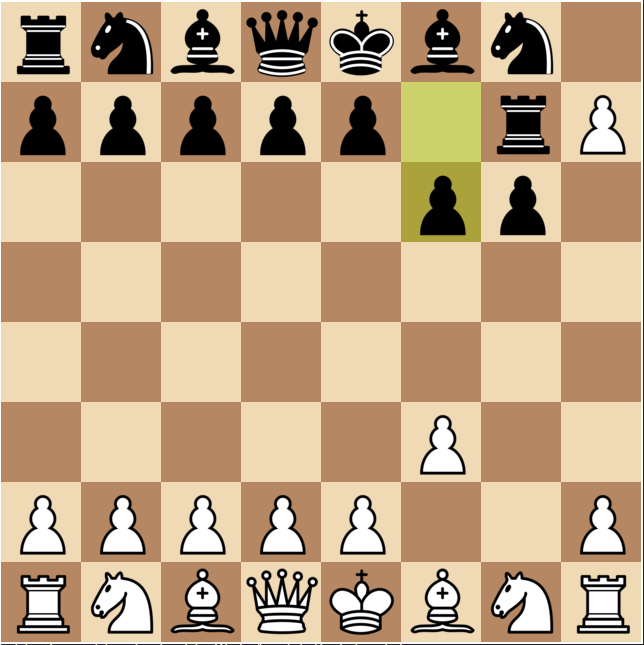
\includegraphics[scale=0.15]{{fig/pre_promotion.png}}
    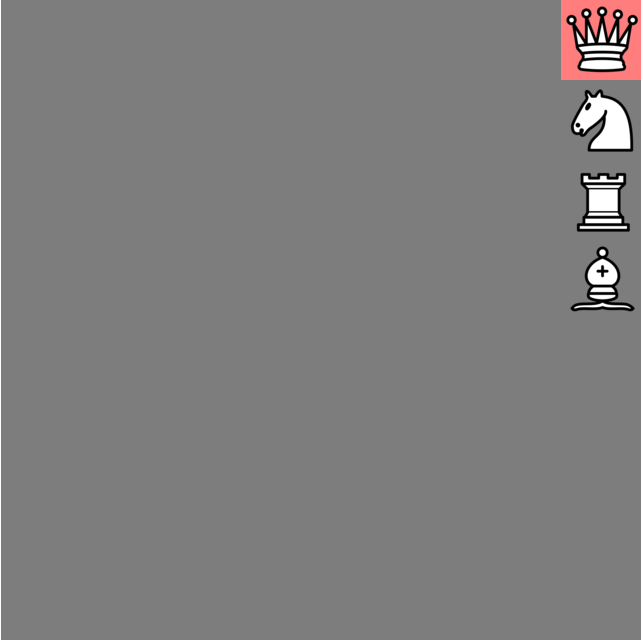
\includegraphics[scale=0.15]{{fig/promoting_pawn.png}}
    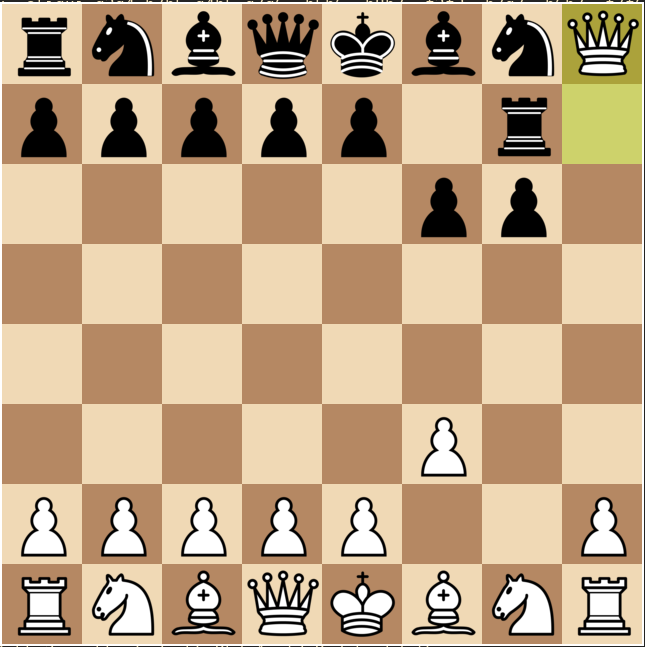
\includegraphics[scale=0.15]{{fig/promoted_pawn.png}}
    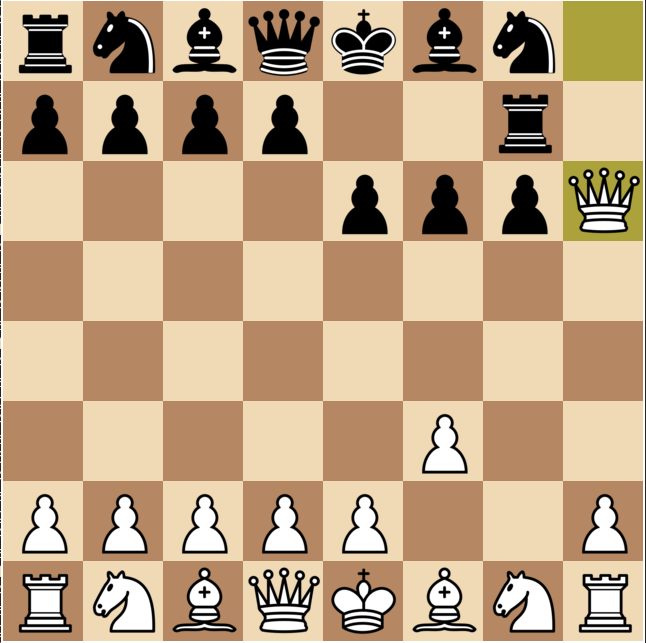
\includegraphics[scale=0.15]{{fig/queen_moving_promotion.png}}
    \caption{Overview of different states of the game while in GUI. With a
    Pawn promoting to a Queen.}
\end{figure}




\end{document}

